\chapter{Results}

\section{Network Training}

The first stage of training was search for the better topology regions. It also involved confirming the best activation functions to use.

\subsection{Optimising Topology and Activation Functions}

Table~\ref{tab:leaky_perf} shows the best networks trained using leaky ReLU in the hidden layers. Learning rates of 0.01, 0.05 and 0.1 were all tested, 0.01 was the best.

\begin {table}[H]
\caption{Leaky ReLU Best performance, lr=0.01} \label{tab:leaky_perf}
\begin{center}
    \begin{tabu}{| r r r r r | }
        \hline
        \rowfont[c]{\bfseries} First & Second & Epochs & Alpha & Loss \\
        \hline\hline
            3 & 2 & 100 & 0.1 & 8.40\% \\ \hline
            4 & 2 & 100 & 0.1 & 8.42\% \\ \hline
            4 & 4 & 100 & 0.1 & 8.47\% \\ \hline
            4 & 4 & 100 & 0.2 & 8.71\% \\ \hline
            2 & 2 & 100 & 0.1 & 9.23\% \\ \hline
            3 & 3 & 100 & 0.1 & 9.95\% \\ \hline
    \end{tabu}
\end{center}
\end{table}

\begin{figure}[H]
\caption{Leaky ReLU performance with Learning Rate 0.01}
\label{fig:leaky}
\centering
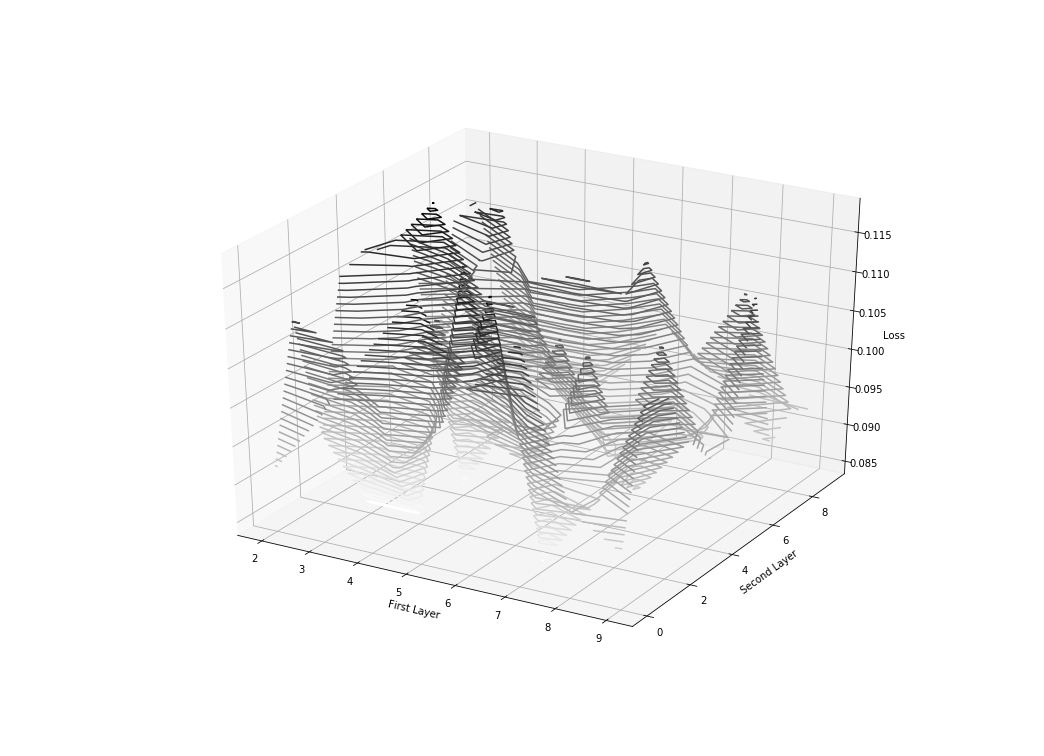
\includegraphics[width=1.0\textwidth]{Figures/leaky.png}
\end{figure}

Table~\ref{tab:tanh_perf} shows the performance when training with the tanh function. Tanh performed very poorly as an activation function on the output layer. Even though tanh is centered around zero, this should not have affected the training as the purpose of the bias unit is to assist in a shift on the y-axis. One possible additional test for this is to re-encode the False signals to $-1$, but given that tanh is a scaled version of sigmoid, sigmoid can be used instead.

\begin {table}[H]
\caption{Tanh Best performance, lr=0.01} \label{tab:tanh_perf}
\begin{center}
    \begin{tabu}{| r r r r r | }
        \hline
        \rowfont[c]{\bfseries} First & Second & Learning Rate & Epochs & Loss \\
        \hline\hline
            2 & 2 & 0.01 & 100 & 106.69\% \\ \hline
            3 & 1 & 0.01 & 100 & 106.69\% \\ \hline
            2 & 1 & 0.01 & 100 & 133.67\% \\ \hline
            2 & 2 & 0.05 & 100 & 149.52\% \\ \hline
            2 & 1 & 0.05 & 100 & 149.52\% \\ \hline
            3 & 1 & 0.05 & 100 & 149.52\% \\ \hline
    \end{tabu}
\end{center}
\end{table}

Using the combination of ReLU as the activation function for hidden layers, and sigmoid as the activation function at the final layer was the best result.

\begin {table}[H]
\caption{Sigmoid Best performance} \label{tab:sigmoid_perf}
\begin{center}
    \begin{tabu}{| r r r r r | }
        \hline
        \rowfont[c]{\bfseries} First & Second & Learning Rate & Epochs & Loss \\
        \hline\hline
            3 & 2 & 0.01 & 56 & 6.03\% \\ \hline
            3 & 1 & 0.01 & 92 & 6.04\% \\ \hline
            5 & 0 & 0.01 & 73 & 6.13\% \\ \hline
            7 & 2 & 0.01 & 50 & 6.13\% \\ \hline
            10 & 2 & 0.01 & 60 & 6.26\% \\ \hline
            4 & 1 & 0.01 & 38 & 6.32\% \\ \hline
            2 & 2 & 0.01 & 73 & 6.32\% \\ \hline
            8 & 0 & 0.05 & 93 & 6.35\% \\ \hline
            6 & 4 & 0.01 & 84 & 6.37\% \\ \hline
            4 & 0 & 0.01 & 100 & 6.38\% \\ \hline
    \end{tabu}
\end{center}
\end{table}

\begin{figure}[H]
\caption{Network Topology affect on Loss Function}
\label{fig:topology_loss}
\centering
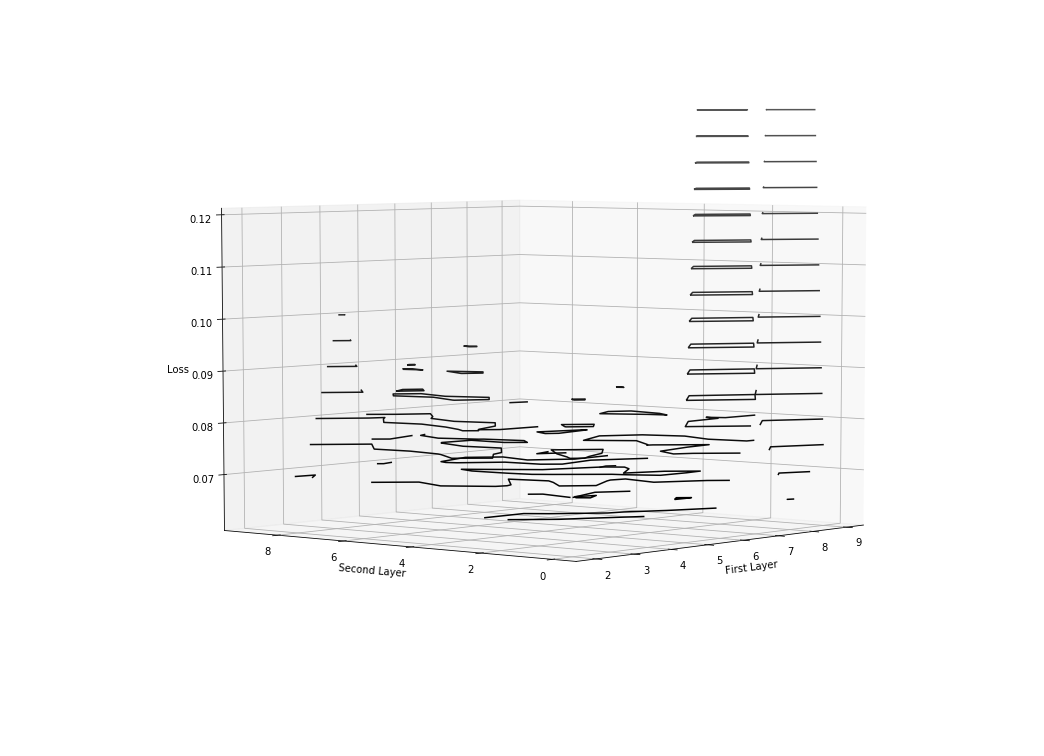
\includegraphics[width=1.0\textwidth]{Figures/sigmoid_chart.png}
\end{figure}

Figure~\ref{fig:nodesVloss}, shows the slight positive correlation ($\rho =0.4$) between the loss function on the test set, and the number of total nodes in a network. This shows the more nodes in a network, the more likely it is to over-fit the data. A simpler, generalised solution is more likely to have predictive power on an unseen data set.

\begin{figure}[H]
    \centering
    \caption{Total Hidden Nodes Vs Loss Function}
    \label{fig:nodesVloss}
        \begin{tikzpicture}
        \begin{axis} [enlargelimits=true, x tick label style={
            /pgf/number format/.cd,
                fixed,
                fixed zerofill,
                precision=0,
                /tikz/.cd
            },
            ymin=0,
            xmin=0,
            xlabel={Total Nodes},
            ylabel={Loss (\%)}
            ]
        \addplot+[
            only marks,
            scatter,
            mark= o,
            mark size=2.9pt]
        table {Data/NodesLR.dat};
        \end{axis}
        \end{tikzpicture}
\end{figure}

\subsection{Hyper-parameters}

The next iteration was to search more possibilities for the learning rate, and also test with a momentum term. Table~\ref{tab:momentum_perf} shows the results using two hidden layers; three nodes in the first hidden layer, and two nodes in the second.

\begin {table}[H]
\caption{Best performance adjusting Momentum} \label{tab:momentum_perf}
\begin{center}
    \begin{tabu}{| r r r r | }
        \hline
        \rowfont[c]{\bfseries} Epochs & Learning Rate & Momentum & Loss \\
        \hline\hline
            35 & 0.010 & 0.6 & 7.99\% \\ \hline
            27 & 0.009 & 0.5 & 8.00\% \\ \hline
            18 & 0.009 & 0.7 & 8.06\% \\ \hline
            25 & 0.011 & 0.7 & 8.06\% \\ \hline
            13 & 0.006 & 0.8 & 8.09\% \\ \hline
    \end{tabu}
\end{center}
\end{table}

\begin{figure}[H]
\caption{Effect of learning rate and momentum on the Loss Function}
\label{fig:leaky}
\centering
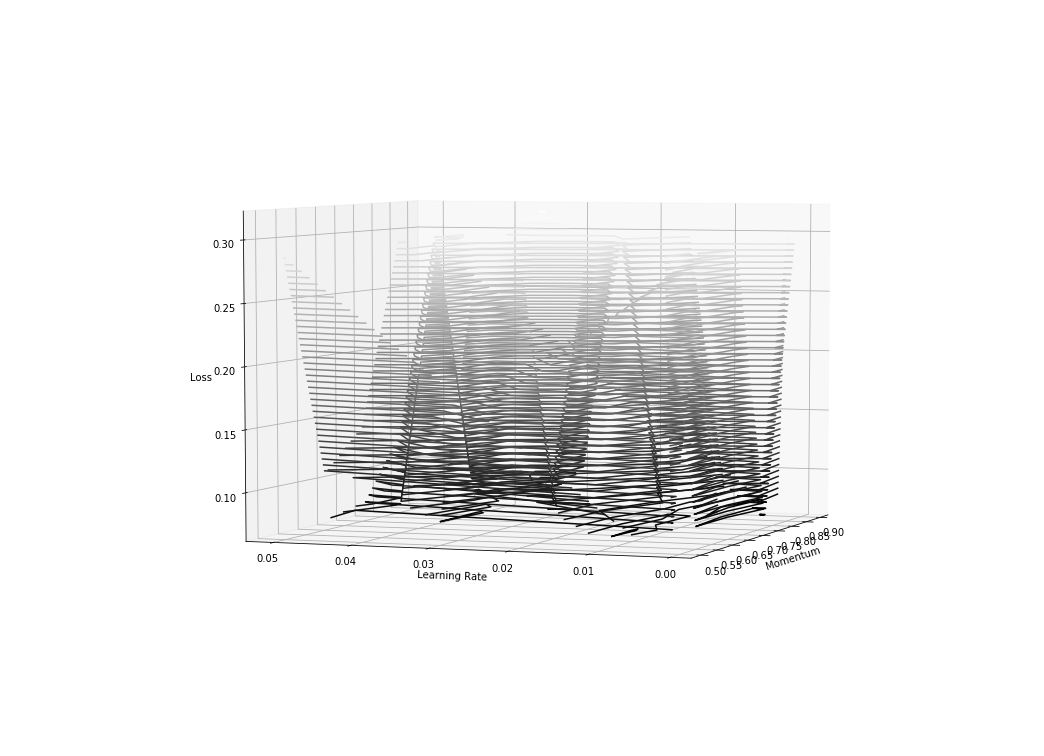
\includegraphics[width=1.0\textwidth]{Figures/momentum_test.png}
\end{figure}

Momentum did not appear to help find a global minimum, but it did help speed the training up, and converge faster.

Focusing on the learning rate, the best rate seemed to be between 0.001 and 0.1 as per Figure~\ref{fig:loss_learn}.

\begin{figure}[H]
\caption{Learning Rate vs Loss}  \label{fig:loss_learn} 
\centering
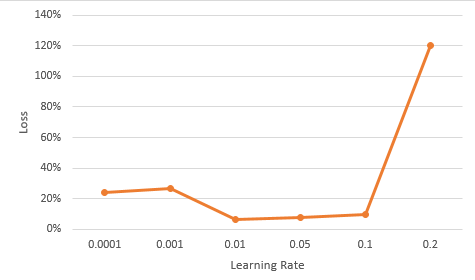
\includegraphics[width=0.8\textwidth]{Figures/LearningRate1.PNG}
\end{figure}

After narrowing the range using the learning rate with no momentum, the results is shown in figure~\ref{fig:narrow_LR}. This shows that the best learning rate for this network is still 0.01.

\begin{figure}[H]
\caption{Narrow Learning Rate Search}  \label{fig:narrow_LR} 
\centering
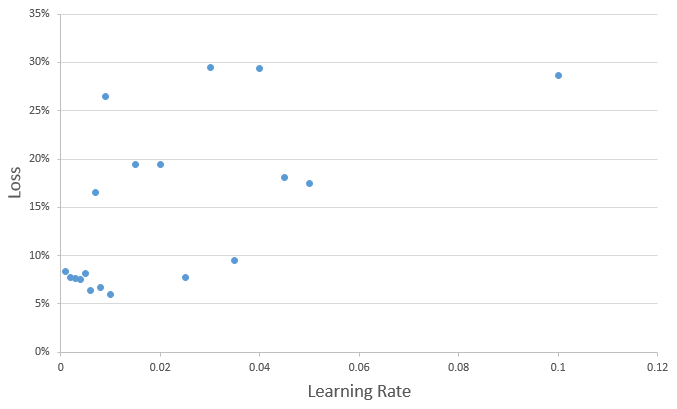
\includegraphics[width=0.8\textwidth]{Figures/LearningRate2.PNG}
\end{figure}

Figure~\ref{fig:learningrate} compares the same model topology, but with a different learning rate. The best performing model tested quickly moved along the cost function and was stopped early. With a much higher learning rate, the second test didn't converge, even after running for 200 epochs.

\begin{figure}[H]
    \centering
    \caption{Evidence of the effect of accurate learning rate}
    \label{fig:learningrate}
        \begin{tikzpicture}
        \begin{axis} [enlargelimits=false,
            y tick label style={
                /pgf/number format/.cd,
                fixed,
                fixed zerofill,
                precision=2,
                /tikz/.cd
            },
            ymin=0,
            xlabel=Epochs,
		    ylabel=Validation Loss,
            ]
        \addplot+[mark= +,
            mark size=2pt
            ]
        table[meta=Oscillates] {Data/LossFunction.dat};
        \addplot+[mark= x,
            mark size=2pt
            ]
        table[meta=Converges] {Data/LossFunction2.dat};
        \legend{$lr=0.2$,$lr=0.01$}
        \end{axis}
        \end{tikzpicture}
\end{figure}

\subsection{Trained Model}

Figure~\ref{fig:modelviz} shows the Keras visualisation of the model with the lowest loss on the test set.

\begin{figure}[H]
\caption{Keras Model vizualisation}  \label{fig:modelviz} 
\centering
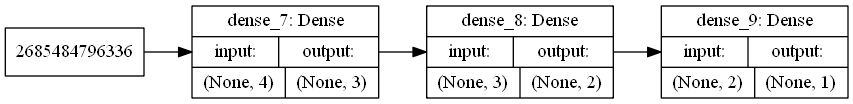
\includegraphics[width=0.8\textwidth]{Figures/model.png}
\source{Keras \cite{chollet2015keras}}
\end{figure}

This same model is graphically displayed in figure \ref{fig:fullmodel}. The weights on each connection of this model are in Table~\ref{tab:weights}.

\begin{sidewaysfigure}
\caption{Final Model Vizualisation}  \label{fig:fullmodel} 
\centering
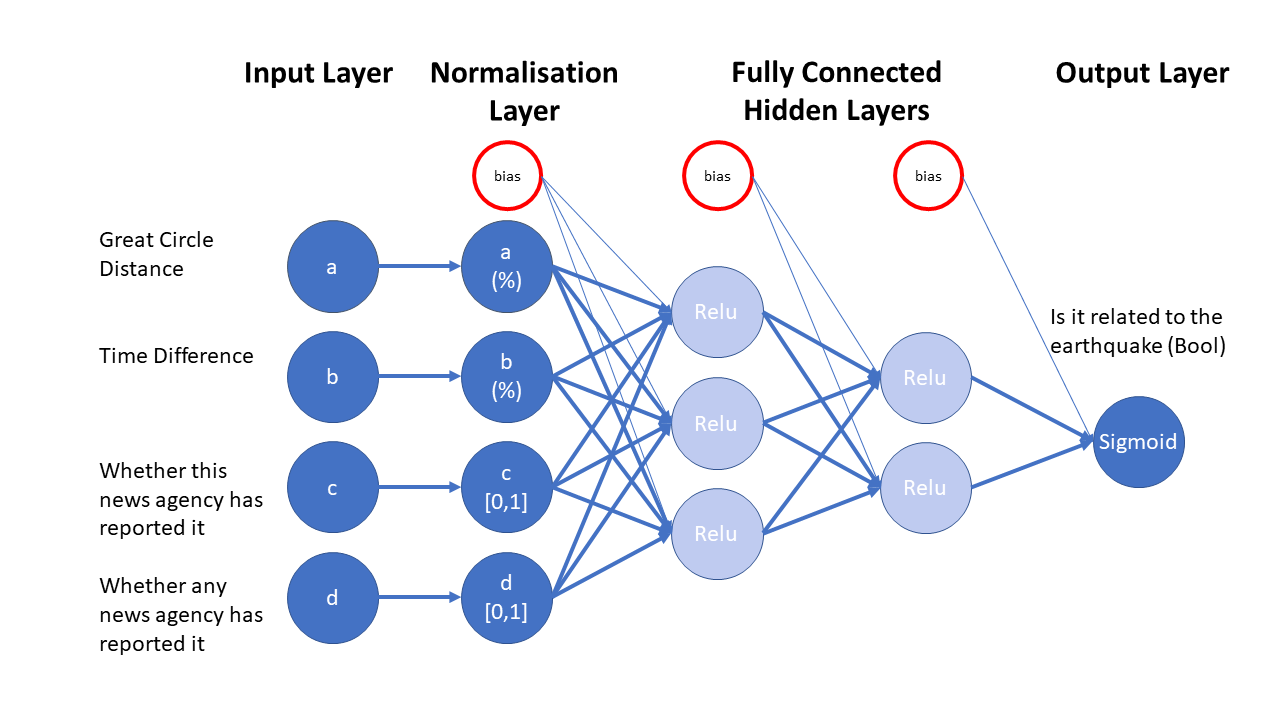
\includegraphics[width=0.9\textwidth]{Figures/FinalNetwork.png}
\end{sidewaysfigure}

\begin {table}[H]
\caption{Best Model Weights} \label{tab:weights}
\begin{center}
\begin{tabu}{l | r r r}
{} & \multicolumn{3}{c}{Nodes} \\
Hidden Layer 1 & 0 & 1 & 2 \\
\hline
0 & -0.64314 & 2.01097 & -0.70205 \\
1 & -0.84878 & 5.35289 & -1.27414 \\
2 & 0.80032 & -0.15045 & -0.23485 \\
3 & 0.02895 & 0.17063 & 0.6392 \\
bias & 0.17831 & 0.06045 & 0.33984 \\
\multicolumn{4}{c}{} \\
{} & \multicolumn{3}{c}{Nodes} \\
Hidden Layer 2 & 0 & 1 & {} \\
\hline
0 & -0.3866 & -1.17079 & {} \\
1 & 2.83778 & 0.99092 & {} \\
2 & -0.90759 & 0.38192 & {} \\
bias & 0.36265 & -0.11841 & {} \\
\multicolumn{4}{c}{} \\
{} & \multicolumn{3}{c}{Nodes} \\
Output & 0 & {} & {} \\
\hline
0 & -2.31861 & {} & {} \\
1 & -1.13171 & {} & {} \\
bias & 2.08073 & {} & {} \\
\end{tabu}
\end{center}
\end{table}

\subsection{Interpreting Predictions}

The objective of training the neural network, was to find a way to systematically predict the sell signal for a trade. Because the system outputs a probability, and the target is a binary, the predictions need to be mapped to a value using thresholding, as discussed in chapter 2.

It is up to the individual practitioner if a decision is required on each tweet. If it is, the standard ROC graph can be used. This ROC graph is shown in figure~\ref{fig:threshold} and shows the relationship between false positives and true positives at different thresholds.

\begin{figure}[H]
    \centering
    \caption{ROC chart for standard threshold tests}
    \label{fig:threshold}
        \begin{tikzpicture}
        \begin{axis} [enlargelimits=false,
            y tick label style={
                /pgf/number format/.cd,
                fixed,
                fixed zerofill,
                precision=2,
                /tikz/.cd
            },
            x tick label style={
                /pgf/number format/.cd,
                fixed,
                fixed zerofill,
                precision=2,
                /tikz/.cd
            },
            ymin=0,
            xmin=0,
            xlabel=fp rate,
		    ylabel=tp rate,
            ]
        \addplot+[mark= +,
            mark size=2pt
            ]
        table[meta=fp_rate] {Data/ROC.dat};
        \addplot+[mark= x,
            mark size=1pt
            ]
        table[meta=tp_rate] {Data/ROC.dat};
        \end{axis}
        \end{tikzpicture}
\end{figure}

In this case, the threshold that produced the largest Area-under-curve was 85\%. This value gave a tp rate of 93.5\% and an fp rate of only 5.3\%, for an AUC of 88.6\%.

Table~\ref{tab:prediction} shows the breakdown of the predictions of the selected model on the testing data set at different threshold levels allowing for an undefined reading. It shows how a wider band not only reduces the errors, but also reduces the accurate predictions.

\begin {table}[H]
\caption{Prediction Precision} \label{tab:prediction}
\begin{center}
    \begin{tabu}{| r r r r r r r | }
        \hline
        \rowfont[c]{\bfseries} Actual & Prediction & 0.5 & $\pm$0.1 & $\pm$0.2 & $\pm$0.3 & $\pm$0.4 \\
        \hline\hline
        FALSE & FALSE & 89.4\% & 88.6\% & 88.3\% & 87.0\% & 86.2\% \\
        TRUE & FALSE & 1.5\% & 0.5\% & 0.3\% & 0.1\% & 0.0\% \\
        FALSE & TRUE & 2.0\% & 0.9\% & 0.4\% & 0.2\% & 0.0\% \\
        TRUE & TRUE & 7.1\% & 6.2\% & 5.9\% & 4.4\% & 0.0\% \\
        \hline
        {} & Total & 100.0\% & 96.3\% & 95.0\% & 91.7\% & 86.2\% \\
        \hline
    \end{tabu}
\end{center}
\end{table}

When plotted, with the adjusted tp, it gives the ROC graph shown in figure~\ref{fig:threshold_adj}.

\begin{figure}[H]
    \centering
    \caption{ROC chart for threshold tests allowing a middle range of un-defined}
    \label{fig:threshold_adj}
        \begin{tikzpicture}
        \begin{axis} [enlargelimits=false,
            y tick label style={
                /pgf/number format/.cd,
                fixed,
                fixed zerofill,
                precision=2,
                /tikz/.cd
            },
            x tick label style={
                /pgf/number format/.cd,
                fixed,
                fixed zerofill,
                precision=3,
                /tikz/.cd
            },
            ymin=0,
            xmin=0,
            xlabel=fp rate,
		    ylabel=tp rate,
            ]
        \addplot+[mark= +,
            mark size=2pt
            ]
        table[meta=fp_rate] {Data/ROC_adj.dat};
        \addplot+[mark= x,
            mark size=1pt
            ]
        table[meta=tp_rate] {Data/ROC_adj.dat};
        \end{axis}
        \end{tikzpicture}
\end{figure}

For this ROC graph, the threshold that produced the largest Area-under-curve was 50$\pm$2\%. This value gave a tp rate of 78.3\% and an fp rate of only 1.3\%, for an AUC of only 77.3\%.

\pagebreak
\section{Data Mining Results}

\subsection{Significant returns against all earthquakes}

Due to the nature of trading hours for many of these instruments, it is very possible that an earthquake happens while markets are closed, and so no one is able to capitalise. As previously discussed FX markets are open 24 hours, 7 days a week, and most commodities are able to be traded in some way during the work week.

Despite this, the below commodity indices have a clear relationship with shock events and prices of base metals tend to drop, straight after an earthquake. Table~\ref{tab:commods_significance_pre} shows that the only indices to move significantly, prior to the USGS tweet are commodities. It is very important to note that these global commodity markets are the first to react to earthquakes. Likely for fundamental reasons such as the potential disruption to supply chains. However, from a trading point of view the return was not worth the risks, as seen by the sharpe ratios less than one.

In this table, and the other tables showing returns, if a return is negative, profits can be made by taking the short position at open and closing the trade with a buy.

\begin {table}[H]
\caption{Significant returns to all earthquakes \textit{before} the USGS tweet} \label{tab:commods_significance_pre}
\begin{center}
    \begin{tabu}{| l l r r r r r | }
        \hline
        \rowfont[c]{\bfseries} Asset & Name & t-stat & p & Rtrn & StDev & Sharpe \\
        \hline \hline
        Commod & SUGAR \#11 (WORLD) & -5.8 & 0.000 & -2.3\% &4.6\% & -0.50 \\
        Commod & LME NICKEL 3MO (\$) & -7.04 & 0.000 & -2.4\% &4.1\% & -0.59 \\
        Commod & Singapore 180 Cst Fuel Month 1 & -5.33 & 0.000 & -1.3\% &3.4\% & -0.39 \\
        Commod & Low Su Gasoil G & -2.81 & 0.006 & -0.4\% &1.5\% & -0.27 \\
        Commod & LME COPPER 3MO (\$) & -2.24 & 0.027 & -0.8\% &4.1\% & -0.20 \\
        Commod & Palladium Spot  \$/Oz & -2.02 & 0.046 & -0.6\% &3.9\% & -0.16 \\
        Commod & GASOLINE RBOB FUTURE & 2.43 & 0.017 & 0.4\% &2.8\% & 0.14 \\
        Commod & ALUMINUM FUTURE & 4.81 & 0.000 & 1.0\% &2.6\% & 0.38 \\
    \hline
    \end{tabu}
    \source{Bloomberg L.P.\cite{bloomberg}}
\end{center}
\end{table}

After the USGS tweet, the base metal prices start to revert after the disruption. Some agricultural commodity markets that didn't move significantly prior to the USGS signal dropped in this second time frame. These trades also had too much risk for the potential return.

\begin {table}[H]
\caption{Significant returns to all earthquakes \textit{after} the USGS tweet.} \label{tab:commods_significance_post}
\begin{center}
    \begin{tabu}{| l l r r r r r | }
        \hline
        \rowfont[c]{\bfseries} Asset & Name & t-stat & p & Rtrn & StDev & Sharpe \\
        \hline \hline
        Commod & WHEAT FUTURE(CBT) & -9.25 & 0.000 & -5.5\% &6.8\% & -0.81 \\
        Commod & CATTLE FEEDER FUTURE & -2.63 & 0.010 & -0.5\% &2.3\% & -0.22 \\
        Commod & COTTON NO.2 FUTURE & -2.03 & 0.045 & -0.7\% &4.2\% & -0.17 \\
        Commod & BRENT CRUDE FUTURE & 1.99 & 0.049 & 0.4\% &2.8\% & 0.14 \\
        Commod & LME COPPER 3MO (\$) & 2.1 & 0.038 & 0.8\% &4.9\% & 0.16 \\
        Commod & Singapore 180 Cst Fuel Month 1 & 5.14 & 0.000 & 1.4\% &3.9\% & 0.36 \\
        Commod & LME NICKEL 3MO (\$) & 6.2 & 0.000 & 2.1\% &4.5\% & 0.46 \\
        Commod & NATURAL GAS FUTURE & 9.71 & 0.000 & 1.4\% &2.7\% & 0.51 \\
        Commod & SUGAR \#11 (WORLD) & 6.01 & 0.000 & 2.5\% &4.8\% & 0.52 \\
    \hline
    \end{tabu}
    \source{Bloomberg L.P.\cite{bloomberg}}
\end{center}
\end{table}

\subsection{Significant Returns against local earthquakes}

Filtering the time series from earthquake to when the USGS announced it by the distance from the epicentre show that equity indices are more susceptible to local movements, than global. 5000km was used as the threshold for nearby indices in the case of the one tailed test. The below indices had more consistent returns as can be seen by the higher sharpe ratios. The Japanese market, through the Nikkei 225 and Nikkei 400, was more susceptible to movements after an earthquake, and with more consistency. Orange juice futures also had more high excess returns for the unit risk.

\begin {table}[H]
\caption{Significant returns to nearby earthquakes} \label{tab:near_eq_significance_pre}
\begin{center}
    \begin{tabu}{| l l r r r r r | }
        \hline
        \rowfont[c]{\bfseries} Asset & Name & t-stat & p & Rtrn & StDev & Sharpe \\
        \hline \hline
        Eq & NIKKEI 225 & 12.21 & 0.000 & 2.5\% &1.6\% & 1.56 \\
        Eq & JPX Nikkei Index 400 & 23.11 & 0.000 & 2.0\% &1.3\% & 1.53 \\
        Commod & FCOJ-A FUTURE & 6.63 & 0.000 & 2.2\% &1.3\% & 1.48 \\
        Eq & NYSE FINANCIAL INDEX & 2.73 & 0.029 & 1.4\% &1.6\% & 0.87 \\
        Eq & TAIWAN TAIEX INDEX & 2.84 & 0.012 & 1.5\% &2.1\% & 0.71 \\
    \hline
    \end{tabu}
    \source{Bloomberg L.P.\cite{bloomberg}}
\end{center}
\end{table}

\subsection{Significant Pair Trades}

Despite this, the experiment was not able to find any significant pair trade ideas by comparing indices located close to the epicenter with those further away.

It is interesting to note that filtering by the magnitude of the earthquake didn't help to produce significant results. Whether grouping by asset class, or looking at individual indices, there was no significant movements when filtered by earthquakes above 6, 6.5 or 7 on the Richter scale.

\subsection{Significant Returns directly after the USGS tweets}

When testing the minute data after the USGS tweet, patterns similar to the first tests emerged. Commodity prices seem to be highly affected by earthquakes, however these ones were large negative movements after the USGS tweet.It usually took over 30 minutes for a significant movement to be found.

\begin {table}[H]
\caption{Asset price changes minute data } \label{tab:minute_data}
\begin{center}
    \hspace*{-2cm}\begin{tabu}{| l l r r r r r r | }
        \hline
        \rowfont[c]{\bfseries} Asset & Name & Minutes & t-stat & p & Rtrn & StDev & Sharpe \\
        \hline \hline
Commod & LME NICKEL 3MO (\$) & 31 & -14.4 & 0.000 & -3.0\% & 2.2\% & -1.37 \\ 
Commod & GASOLINE RBOB FUTURE & 33 & -13.7 & 0.000 & -3.4\% & 2.6\% & -1.29 \\ 
Commod & WHEAT FUTURE(CBT) & 40 & -12.6 & 0.000 & -8.0\% & 6.7\% & -1.2 \\ 
Commod & CORN FUTURE & 40 & -12.2 & 0.000 & -6.0\% & 5.2\% & -1.15 \\ 
Commod & NY Harb ULSD Future & 40 & -11.3 & 0.000 & -1.4\% & 1.3\% & -1.07 \\ 
Commod & ZINC FUT (SHFE) & 35 & -11.0 & 0.000 & -5.6\% & 5.3\% & -1.06 \\ 
Commod & WTI CRUDE FUTURE & 38 & -10.1 & 0.000 & -1.1\% & 1.2\% & -0.96 \\ 
Commod & ALUMINUM FUTURE & 40 & -8.3 & 0.000 & -1.5\% & 1.8\% & -0.82 \\ 
Commod & FCOJ-A FUTURE & 40 & -6.4 & 0.000 & -1.1\% & 1.8\% & -0.63 \\ 
Commod & BRENT CRUDE FUTURE & 38 & -6.3 & 0.000 & -0.7\% & 1.1\% & -0.61 \\ 
Commod & NATURAL GAS FUTURE & 40 & -5.1 & 0.000 & -1.0\% & 2.0\% & -0.49 \\ 
Commod & SUGAR \#11 (WORLD) & 40 & -4.3 & 0.000 & -1.4\% & 3.2\% & -0.42 \\ 
Commod & Palladium Spot  \$/Oz & 33 & -3.2 & 0.002 & -1.1\% & 3.7\% & -0.3 \\ 
Commod & COFFEE 'C' FUTURE & 38 & -2.9 & 0.004 & -1.4\% & 4.9\% & -0.29 \\ 
Commod & Deformed Bar Future & 40 & -2.3 & 0.022 & -1.3\% & 5.7\% & -0.22 \\ 
Commod & SILVER FUTURE & 38 & -2.2 & 0.028 & -0.7\% & 3.3\% & -0.22 \\ 
Commod & Silver Spot  \$/Oz & 38 & -2.2 & 0.033 & -0.6\% & 3.0\% & -0.21 \\ 
Commod & PALLADIUM FUTURE & 39 & 2.3 & 0.022 & 0.7\% & 3.3\% & 0.22 \\ 
    \hline
    \end{tabu}
    \source{Bloomberg L.P.\cite{bloomberg}}
    \hspace*{-2cm}
\end{center}
\end{table}

%chart of returns per minute?
These results are promising, and show that there can be excess returns gained from trading signals generated through earthquake analysis.




%In the Results chapter  describe and summarize the results  found.
%² Remember to include comments that remind r committee that r results satisfy r research objectives and research scope.
%² Whenever possible, use graphical methods to summarize results. For example, it is difficult to see patterns with tables. Results in tables should be supplemented with graphs, plots, ¯gures, ...
%² When presenting speci¯c results,  should mention the research objective that is related to those results.
%² By the end of the Results chapters,  want r committee to know that  have satis¯ed all research objectives and research scope.
